\documentclass[conference]{IEEEtran}
\IEEEoverridecommandlockouts
% The preceding line is only needed to identify funding in the first footnote. If that is unneeded, please comment it out.
\usepackage{cite}
\usepackage{amsmath,amssymb,amsfonts}
\usepackage{algorithmic}
\usepackage{graphicx}
\usepackage{textcomp}
\usepackage{pdfpages}
\usepackage{xcolor}
\usepackage{svg}
\usepackage{float}
\usepackage{hyperref}
\usepackage{tikz}
\usepackage{url}
\usepackage{graphicx}
\usepackage{dblfloatfix}

\hypersetup{
    colorlinks,
    citecolor=black,
    filecolor=black,
    linkcolor=black,
    urlcolor=black,
    pdftitle={EE314 Project Final Report}
}

\makeatletter % changes the catcode of @ to 11
\newcommand{\linebreakand}{%
  \end{@IEEEauthorhalign}
  \hfill\mbox{}\par
  \mbox{}\hfill\begin{@IEEEauthorhalign}
}
\makeatother % changes the catcode of @ back to 12


\def\BibTeX{{\rm B\kern-.05em{\sc i\kern-.025em b}\kern-.08em
    T\kern-.1667em\lower.7ex\hbox{E}\kern-.125emX}}

\begin{document}

\title{EE 314 DIGITAL CIRCUITS LABORATORY 2022-2023 SPRING TERM PROJECT REPORT \\ {\large FPGA IMPLEMANTATION OF A 2D STRATEGY GAME}}

\author{\IEEEauthorblockN{Ahmet Caner Akar}
\IEEEauthorblockA{\textit{Electrical and Electronics Engineering Department} \\
\textit{Middle East Technical University}\\
Ankara, Turkey \\
e244228@metu.edu.tr}
\and
\IEEEauthorblockN{Osama Awad}
\IEEEauthorblockA{\textit{Electrical and Electronics Engineering Department} \\
\textit{Middle East Technical University}\\
Ankara, Turkey \\
e248849@metu.edu.tr}
\and
\linebreakand
\IEEEauthorblockN{İsmail Enes Bülbül}
\IEEEauthorblockA{\textit{Electrical and Electronics Engineering Department} \\
\textit{Middle East Technical University}\\
Ankara, Turkey \\
e244263@metu.edu.tr}
}

\maketitle

\begin{abstract}
This document is about the end-term project of EE314 Digital Circuits Laboratory, implementation of a 2D strategy game by using FPGA.  \\
\end{abstract}

\begin{IEEEkeywords}
FPGA, Verilog HDL, VGA driver, button debouncing, state-machine
\end{IEEEkeywords} 

\section{Introduction}
\section{Project Overview}
\subsection{VGA Module}
In this project, we are expected to use the VGA interface of the FPGA to display the game board and some information related to the game. 
To do this, we decided to display the game with 640x480 resolution at 60 Hz. \cite{vga} The timing diagram is shown in the figure below.
\begin{figure}[H]
  \centerline{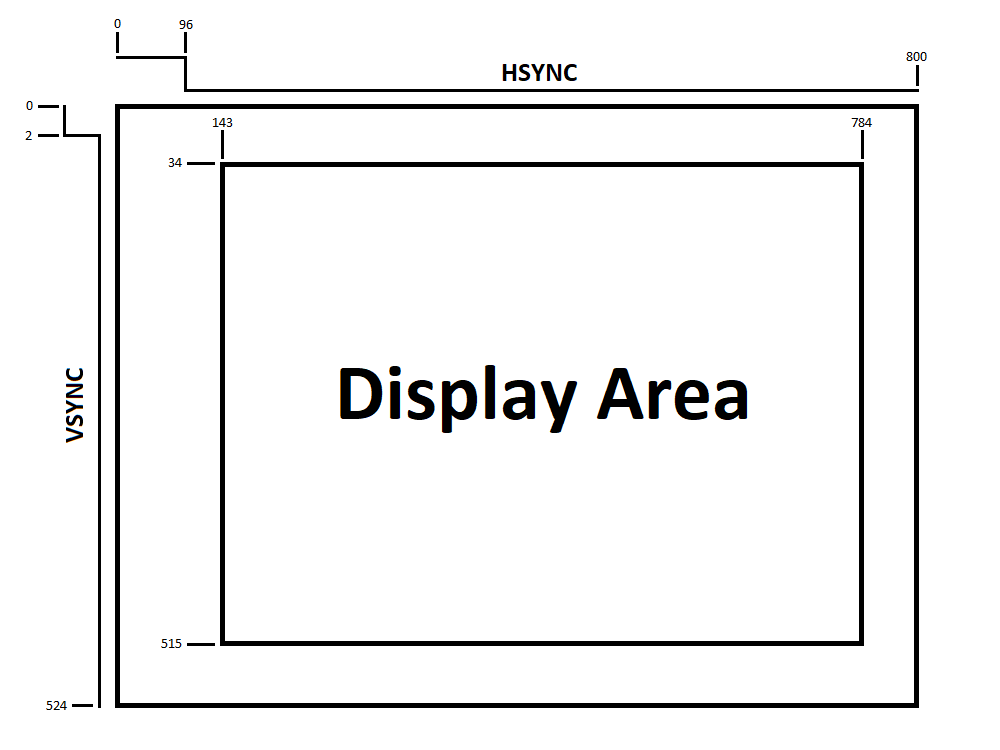
\includegraphics[scale=0.4]{vga.png}}
   \caption{Timing diagram for the VGA interface}
   \label{Fig. 1.}
\end{figure} 
From the timing diagram, we can see that we need two counters namely a horizontal counter and a vertical counter.
To drive counters we need a clock with 25 MHz frequency. 
To obtain a clock signal with that frequency from the internal clock of the FPGA which has a 50 MHz frequency we implemented a clock divider circuit. 
After we obtained the clock signal with a 25 MHz frequency, we connected it to the horizontal counter. 
Horizontal counter counts at every clock cycle, and it counts from 0 to 800. Vertical counter counts 1 when the horizontal counter hits 800. 
We have two synchronization outputs namely HYSNC and VSYNC to tell the monitor beginning and ending of a row and frame respectively. 
HSYNC is high when the horizontal counter is between 0 and 96, and VSYNC is high when the vertical counter is between 0 and 2. 
Altera FPGA uses a digital-to-analog converter that takes 8-bit input for each color channel and converts it to an analog signal that has a voltage between 
0 and 5 Volts. \cite{fpga} \\
\par When the horizontal counter is between 143 and 784, and the vertical counter is between 34 and 515, RGB values of the pixel at the point (hcounter - 143, ycounter - 34) are returned to the DAC of the FPGA. 
We implemented a \textit{rgbSelector} module to get the RGB values for a given coordinate on the display. 
If the given coordinate is in the board region, the module finds the corresponding block coordinate and reads which piece is 
placed to that coordinate from the memory. Then it gets the RGB value from the memory module that corresponds to the piece. 
If the given coordinate is not in the board region but in a region that involves a text or picture, it reads the RGB value from the corresponding memory. 
If it is neither in the board region nor a picture or text region, then it returns a white color. \\
\par Since we need only 5 colors (white, black, red, green, and blue), we encoded and stored pictures that we used with 1 bit for each color channel. 
After the \textit{rgbSelector} module returns RGB values with 1 bit for each channel, 
another module we called \textit{vgaDecoder} converts it to output with 8 bits for each color channel and returns it to the DAC of the FPGA. \\
\par When the counters are not in the display area, 0 is returned to the DAC of the FPGA. 
An example of the display is shown in the figure below.  
\begin{figure}[H]
  \centerline{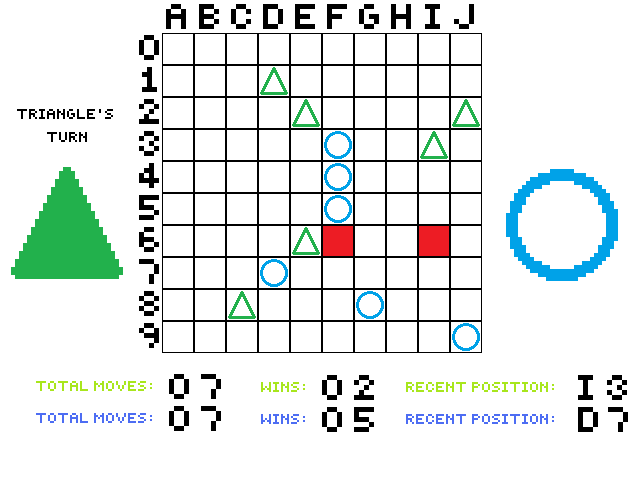
\includegraphics[scale=0.65]{sample_board.png}}
   \caption{Example of the display}
   \label{Fig. 1.}
\end{figure} 
\subsection{Button Debouncing and Edge Detector}
In this project, we need to get three inputs, \textbf{logic 1}, \textbf{logic 0}, and \textbf{activity}, from the user by using push buttons on the FPGA. However, due to mechanical and physical issues, pushbuttons often generate noisy signals called dirty bounces, and these bounces prevent us from properly triggering the program. Thus, to eliminate these undesirable effects, we used the \textit{debouncer\_delayed} module that makes a noisy pushbutton input signal to the ideal input case. \\
\par The working principle of the \textit{debouncer\_delayed} module is quite simple. When a button is pressed, the timer is going to count the elapsed time up to a predefined threshold parameter. If the timer hits the threshold value, the program concludes that the button has reached its steady state and has been pressed. Similarly, when the button is released and the steady state is reached, the program concludes that the button has been released. \\
\par After debouncing the button input, we designed another module called \textit{edge\_detector} to detect the negative and positive edges of the debounced input so that we will use the edge signals directly as button signals in the game controller. \\
\par The \textit{button} module contains both \textit{debouncer\_delayed} and \textit{edge\_detector} modules so that the hierarchical design principle is followed throughout the project. Also, both of these modules, are written like a state machine to make it easier to implement condition-based and flexible code. The waveform simulation result of the \textit{button} module in Quartus II is given in Figure \ref{Fig. 1.}, below. Besides these, in the \textit{button\_top} module each button is defined separately in a hierarchical manner by using the \textit{button} module.
 \begin{figure}[H]
   \centerline{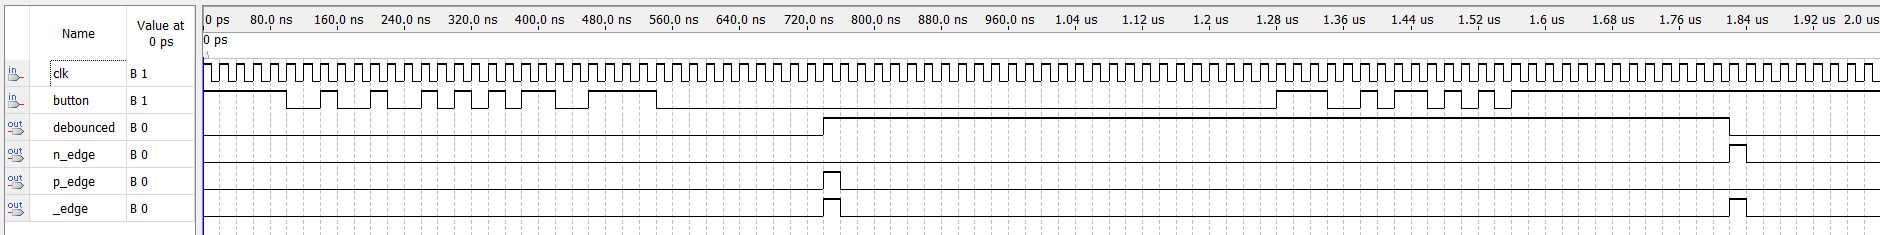
\includegraphics[scale=0.22]{simulation.png}}
    \caption{Button module, waveform simulation result}
    \label{Fig. 1.}
\end{figure} 
\subsection{Game Controller}
   \begin{center}
   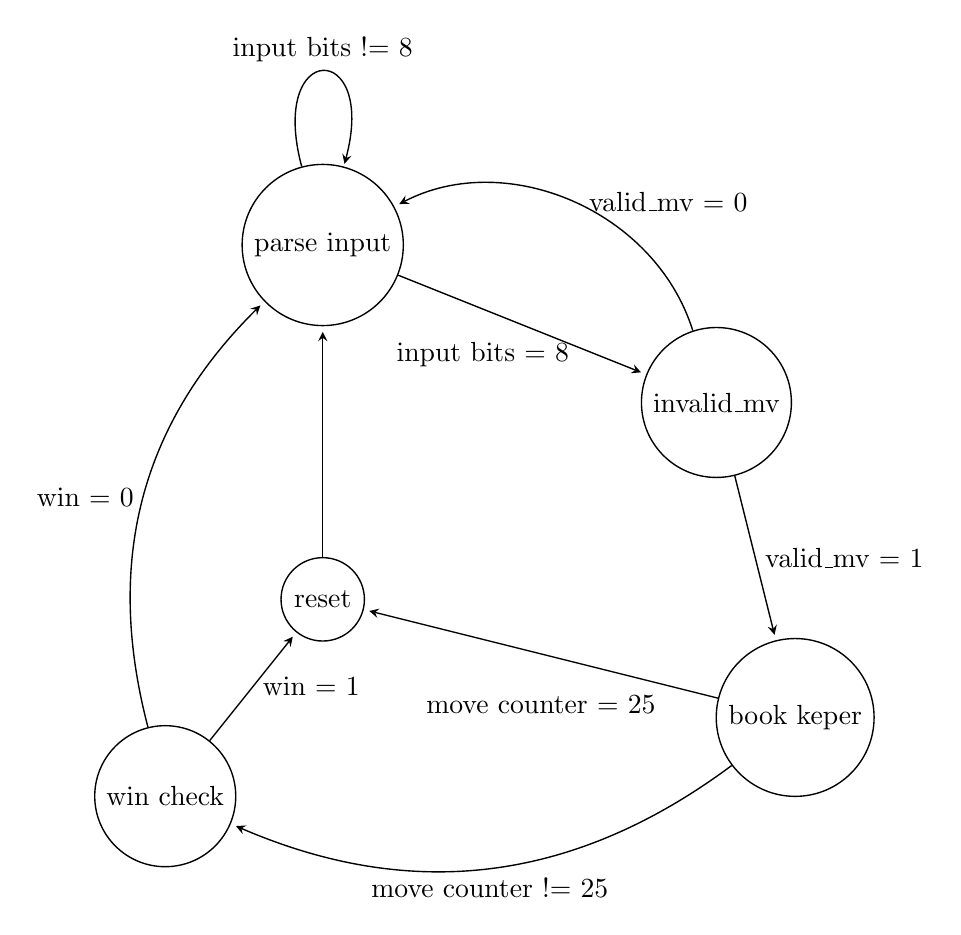
\begin{tikzpicture}[ - > , >= stealth, shorten >=2pt , line width =0.5 pt , node distance =2 cm]
   \node [circle , draw] (parse) at (0 , 0) {parse input};
   \node [circle , draw] (invalid) at (5 , -2) {invalid\_mv};
   \node [circle , draw] (book) at (6 , -6) {book keper};
   \node [circle , draw] (reset) at (0 , -4.5) {reset};
   \node [circle , draw] (win) at (-2 , -7) {win check};
  
   \path (parse) edge [loop above] node [above] {input bits != 8} (parse) ;
   \path (invalid) edge [bend right=50] node [right, xshift=0.1cm] {valid\_mv = 0} (parse) ;
   \path (book) edge [bend left] node [below] {move counter != 25} (win) ;
   \path (win) edge [bend left] node [left] {win = 0} (parse) ;
   \path (win) edge node [right] {win = 1} (reset) ;
   \path (parse) edge node [below, xshift=-0.5cm, yshift=-0.1cm] {input bits = 8} (invalid) ;
   \path (book) edge node [below, yshift=-0.4cm] {move counter = 25} (reset) ;
   \path (invalid) edge node [right] {valid\_mv = 1} (book) ;
   \path (reset) edge node [above] {} (parse) ;
   \end{tikzpicture}
   \end{center}

\section{Conclusion}

\bibliographystyle{ieeetr}
\bibliography{refs}
\end{document}
